\documentclass[journal]{IEEEtran}
\usepackage{subfigure}
\usepackage{cite}
\usepackage{citesort}
\usepackage{amsmath,epsfig,bm}
\usepackage{pifont}
\usepackage{paralist}
\usepackage{graphicx}
\usepackage{amssymb}
\usepackage{amsmath}
\usepackage{cancel}
\usepackage[normalem]{ulem}
\usepackage[dvips]{color}
\usepackage{algorithm}
\DeclareMathOperator*{\argmax}{argmax}
\DeclareMathOperator*{\argmin}{argmin}
\DeclareMathOperator*{\limit}{lim}
\usepackage{pifont}
\usepackage{graphicx}
\usepackage{amssymb}
\usepackage{amsmath}
\usepackage{cancel}
\usepackage[normalem]{ulem}
\usepackage[dvips]{color}
\usepackage{algorithm}
\usepackage{algorithmic}
%\usepackage[titletoc]{appendix}
\newcommand{\INPUT}{\item[\algorithmicinput]}
\newcommand{\algorithmicinput}{\textbf{Input:}}
\newcommand{\OUTPUT}{\item[\algorithmicoutput]}
\newcommand{\algorithmicoutput}{\textbf{Output:}}
\newcommand{\Rho}{\mathrm{P}}

\newtheorem{theorem}{\noindent \textbf{Theorem}}
\newtheorem{lemma}{\noindent \textbf{Lemma}}
\newtheorem{definition}{\noindent \textbf{Definition}}
\newtheorem{proposition}{\noindent \textbf{Proposition}}
\newtheorem{remark}{\noindent \textbf{Remark}}
\newtheorem{corollary}{\noindent \textbf{Corollary}}
%%%%%%%%%%%%%%%%%%%%%%%%%%%%%%%%%%%%%%%%%%%%%%%%%

\hyphenation{op-tical net-works semi-conduc-tor}


\begin{document}

\title{On Different Artificial-Noise Aided Transmission Schemes in MISOME Wiretap Channels}

\author{Shihao Yan, Ramanan Subramanian, Nan Yang, Ingmar Land, Robert Malaney, and Jinhong Yuan}

\maketitle

\begin{abstract}
The problem of achieving secure transmission in a multi-input single-output multi-eavesdropper (MISOME) wiretap channel is considered. It is assumed that the eavesdropper's instantaneous channel-state information (CSI) is unknown, and that both the transmitter-to-legitimate-receiver and transmitter-to-eavesdropper channels exhibit block-Rayleigh fading. 

 under the condition that the eavesdropper's instantaneous channel-state information is unknown to the transmitter and legitimate receiver. \end{abstract}

\section{Introduction}
\section{System Model}

We consider an MISOME wiretap channel where the communication
between the $N$-antenna transmitter (Alice) and the single antenna
receiver (Bob) is overheard by the $M$-antenna malicious eavesdropper
(Eve). In this wiretap channel, we denote the main channel between
Alice and Bob as an $1\times{}N$ vector $\mathbf{f}$ and denote the
eavesdropper's channel between Alice and Eve as an $M \times N$
matrix $\mathbf{G}$. The entries of $\mathbf{f}$ and $\mathbf{G}$ are modeled as
independent and identically distributed (i.i.d.) Rayleigh fading.
Of course, we preserve the practical assumption that the main
channel and the eavesdropper's channel have different average SNRs.
Moreover, we assume that both the main channel and the
eavesdropper's channel are subject to block fading with equal block length. We
further assume that $N > M$ since Eve is able to remove the artificial
noise signals if $N \leq M$ \cite{Zhou}. In this wiretap channel, we
consider that the instantaneous information of $\mathbf{G}$ is not
available to Alice. Moreover, we consider that $\mathbf{f}$ is
precisely estimated by Bob and fed back to Alice. We further
consider that $\mathbf{f}$ is perfectly available at Eve since the
feedback from Bob to Alice is not secure.

We next detail the secure data transmission using artificial noise
in the MISOME wiretap channel. In this wiretap channel, Alice
transmits an information signal $s_{\textrm{I}}$ in conjunction with
an $\left(N-1\right)\times1$ artificial noise signal vector
$\mathbf{s}_{\textrm{N}}$ to Bob, where $s_{\textrm{I}}$ has the
variance $\chi_{\textrm{I}}$ and each entry of
$\mathbf{s}_{\textrm{N}}$ has the variance $\chi_{\textrm{N}}$
\cite{Zhou}. We assume that the total transmit power used by Alice
is $P_{\textrm{T}}$. We denote the fraction of the power allocated
to $s_{\textrm{I}}$ by $\phi$ such that
$\chi_{\textrm{I}}=\phi{}P_{\textrm{T}}$, where $0<\phi\leq{}1$.
Since Alice does not have the access of $\mathbf{G}$, she equally
distributes the transmit power to each entry of
$\mathbf{s}_{\textrm{N}}$ such that
$\chi_{\textrm{N}}=\left(1-\phi\right)P_{\textrm{T}}/\left(N-1\right)$.
In order to transmit $s_{\textrm{I}}$ and $\mathbf{s}_{\textrm{N}}$,
Alice designs an $N\times{}N$ beamforming matrix $\mathbf{V}$ given
by
\begin{align}\label{beamforming_matrix}
\mathbf{V}=\left[\textbf{v}_{\textrm{I}}~\textbf{V}_{\textrm{N}}\right],
\end{align}
where $\textbf{v}_{\textrm{I}}$ is used to transmit $s_{\textrm{I}}$
and $\textbf{V}_{\textrm{N}}$ is used to transmit
$\mathbf{s}_{\textrm{N}}$. The aim of $\mathbf{V}$ is to degrade the
eavesdropper's channel quality by transmitting
$\mathbf{s}_{\textrm{N}}$ in all directions except towards Bob. To
determine $\mathbf{V}$, Alice performs the eigenvalue decomposition
of $\mathbf{F}\triangleq\mathbf{f}^{H}\mathbf{f}$. Then Alice
chooses $\textbf{v}_{\textrm{I}}$ as the principal eigenvector
corresponding to the largest eigenvalue of $\mathbf{F}$ and chooses
$\textbf{V}_{\textrm{N}}$ as the remaining $N-1$ eigenvectors of
$\mathbf{F}$ such that $\textbf{V}_{\textrm{N}}$ lies in the
nullspace of $\textbf{h}^{H}$. Therefore, the $N\times1$ transmitted
signal vector at Alice, $\mathbf{x}$, is given by
\begin{align}\label{transmitted_signal}
\mathbf{x}=\left[\textbf{v}_{\textrm{I}}~\textbf{V}_{\textrm{N}}\right]\left[\begin{array}{c}
s_{\textrm{I}}\\
\mathbf{s}_{\textrm{N}}\end{array}\right]
=\textbf{v}_{\textrm{I}}s_{\textrm{I}}+\textbf{V}_{\textrm{N}}\mathbf{s}_{\textrm{N}}.
\end{align}
According to \eqref{transmitted_signal}, the received signal at Bob
is given by
\begin{align}\label{Receive_Bob}
y=\mathbf{f}\mathbf{x}+n_{\textrm{B}}=\mathbf{f}\textbf{v}_{\textrm{I}}s_{\textrm{I}}+n_{\textrm{B}},
\end{align}
where $n_{\textrm{B}}$ is additive white Gaussian noise (AWGN) at
Bob satisfying
$\mathbb{E}\left[n_{\textrm{B}}n_{\textrm{B}}^{H}\right]=\sigma_{\textrm{B}}^{2}$.
Based on \eqref{Receive_Bob}, the instantaneous received SNR at Bob
is given by
\begin{align}\label{SNR_Bob}
\gamma_{\textrm{B}}=\phi\overline\gamma_{\textrm{B}}\left\|\mathbf{f}\right\|^{2},
\end{align}
where
$\overline\gamma_{\textrm{B}}=P_{\textrm{T}}/\sigma_{\textrm{B}}^{2}$.
According to \eqref{transmitted_signal}, the received signal at Eve
is given by
\begin{align}\label{Receive_Eve}
\mathbf{z}=\mathbf{G}\mathbf{x}+\mathbf{n}_{\textrm{E}}
=\mathbf{G}\textbf{v}_{\textrm{I}}s_{\textrm{I}}+
\mathbf{G}\textbf{V}_{\textrm{N}}\mathbf{s}_{\textrm{N}}+\mathbf{n}_{\textrm{E}},
\end{align}
where $\mathbf{n}_{\textrm{E}}$ is the $M\times{1}$ AWGN vector at
Eve satisfying
$\mathbb{E}\left[\textbf{n}_{\textrm{E}}\textbf{n}_{\textrm{E}}^{H}\right]
=\sigma_{\textrm{E}}^{2}\textbf{I}_{M}$. It is crucial to clarify
that although Eve knows the exact instantaneous knowledge of
$\mathbf{f}$ and $\mathbf{V}$, she cannot eliminate the interference
caused by $\textbf{V}_{\textrm{N}}\mathbf{s}_{\textrm{N}}$ if $N>M$.
As such, the optimal received signal combiner chosen by Eve is a
minimum mean-square error (MMSE) combiner, which gives the maximum
received signal-to-interference-plus-noise ratio (SINR) \cite{Gao}.
Based on \eqref{Receive_Eve}, the instantaneous received SINR at Eve
is given by
\begin{align}\label{SNR_Eve}
\gamma_{\textrm{E}}=\phi\textbf{v}_{\textrm{I}}^{H}\mathbf{G}^{H}\left(\frac{1-\phi}{N-1}\mathbf{G}\textbf{V}_{\textrm{N}}\textbf{V}_{\textrm{N}}^{H}\mathbf{G}^{H}+\frac{1}{\overline\gamma_{\textrm{E}}}\mathbf{I}_{M}\right)^{-1}\mathbf{G}\textbf{v}_{\textrm{I}},
%\gamma_{\textrm{E}}=\frac{\phi\overline\gamma_{\textrm{E}}\left\|\mathbf{G}\textbf{v}_{\textrm{I}}\right\|^{2}}{\left(\frac{1-\phi}{N-1}\right)\overline\gamma_{\textrm{E}}\left\|\mathbf{G}\textbf{V}_{\textrm{N}}\right\|^{2}+1},
\end{align}
where
$\overline\gamma_{\textrm{E}}=P_{\textrm{T}}/\sigma_{\textrm{E}}^{2}$.
In the wiretap channel, we assume that
$\overline\gamma_{\textrm{B}}$ and $\overline\gamma_{\textrm{E}}$
are publicly known. If Alice does not know them, she is still able
to perform the secure data transmission using artificial noise but
not able to calculate the secrecy performance metrics.

Based on \eqref{SNR_Bob}, the CDF of $\gamma_{\textrm{B}}$ is
obtained as
\begin{align}\label{CDF_SNR_Bob}
F_{\gamma_{B}}\left(\gamma\right)=1-e^{-\frac{\gamma}{\phi\overline\gamma_{\textrm{B}}}}
\sum_{n=0}^{N-1}\frac{1}{n!}\left(\frac{\gamma}{\phi\overline\gamma_{\textrm{B}}}\right)^{n}.
\end{align}
Based on \eqref{SNR_Eve}, we find that the entries
of $\mathbf{G}\mathbf{V}$ are i.i.d. zero-mean complex Gaussian
random variables since the entries of $\mathbf{G}$ are i.i.d.
zero-mean complex Gaussian random variables and $\mathbf{V}$ is a
unitary matrix. With the aid of \cite{Gao}, the CDF of
$\gamma_{\textrm{E}}$ is obtained as
\begin{align}\label{CDF_SNR_Eve_MISOME}
F_{\gamma_{E}}\left(\gamma\right)=1&-\frac{e^{-\frac{\gamma}{\phi\overline\gamma_{\textrm{E}}}}}{\left(1+\frac{\left(1-\phi\right)\gamma}{\phi\left(N-1\right)}\right)^{N-1}}
\sum_{p=1}^{M}\frac{1}{\Gamma\left(p\right)}\left(\frac{\gamma}{\phi\overline\gamma_{\textrm{E}}}\right)^{p-1}\notag \\
&~~~~\times \sum_{q=0}^{M-p}{N-1\choose
q}\left(\frac{\left(1-\phi\right)\gamma}{\phi\left(N-1\right)}\right)^{q}.
\end{align}


\section{Three Different Transmission Schemes}

In this section, we first present the details of three different coding and transmission schemes. We then formalize the optimization procedure of the power allocation parameter $\phi$ and different wiretap code rates (e.g., $R_E$, $R_S$) for the three schemes. We also provide some analysis for the optimization of each scheme.

\subsection{On-Off Transmission Scheme}

In the on-off transmission scheme, both $\phi$ and $R_s$ are fixed for each pair of $\overline{\gamma}_B$ and $\overline{\gamma}_E$. We choose $R_B$ as $R_B = C_B$ and thus we have $R_E = C_B - R_s$. Alice only transmit signals when $C_B > R_s$, and thus the transmission probability of the on-off transmission scheme is
\begin{align}
P^{tx}_o(\phi, R_s) = \Pr(C_B > R_s) = 1-F_{\gamma_B}\left(2^{R_s}-1\right).
\end{align}
The secrecy outage probability conditioned on a transmission of the on-off transmission scheme is given by
\begin{align}
P^{so}_o(\phi, R_s) &= \Pr(C_E > R_E|C_B > R_s)\notag \\
%&= \Pr(C_B - C_s > C_B - R_s|C_B > R_s) \notag \\
%& = \frac{\Pr(C_s<R_s<C_B)}{\Pr(C_B>R_s)}\notag \\
%&= \frac{\Pr(C_B>R_s) - \Pr(R_s<C_s)}{\Pr(C_B>R_s)}\notag \\
&= 1 - \frac{1 - \Pr(C_s<R_s)}{P^{tx}_o(\phi, R_s)}
\end{align}
where $\Pr(C_s<R_s)$ is the traditional secrecy outage probability, which has been derived in Jonas's MISOME paper.
The average secrecy rate of the on-off transmission scheme over all realizations of $\gamma_B$ for a given $\overline{\gamma}_B$ is
\begin{align}
\mathcal{R}_o (\phi, R_s) = R_s P^{tx}_o(\phi, R_s).
\end{align}

In the on-off transmission scheme, we intend to optimize $\phi$ and $R_s$ through maximizing $\mathcal{R}_o (\phi, R_s)$ subjective to a given secrecy outage probability. Mathematically, the optimization problem in the on-off transmission scheme is presented as
\begin{align}\label{opt_on_off}
(\phi^{\ast}, R_s^{\ast}) \!=\! \argmax_{0< \phi \leq 1, R_s} \mathcal{R}_o (\phi, R_s), ~\text{s.t.}~ P^{so}_o(\phi, R_s) \leq p_0.
\end{align}

In Fig.~\ref{fig:opt_onoff}, we plot $\mathcal{R}_o (\phi, R_s)$ and $P^{so}_o(\phi, R_s)$ with and without the constraint $P^{so}_o(\phi, R_s) \leq p_0$. We note that $\mathcal{R}_o (\phi, R_s)$ is not a monotonic function of $R_s$ and thus in the optimization presented in \eqref{opt_on_off} we may not have $P^{so}_o(\phi, R_s) = p_0$ for a large $p_0$ (e.g., $p_0 \rightarrow 1$). However, for a small $p_0$ (e.g., $p_0 = 0.1$) we still have $P^{so}_o(\phi, R_s) = p_0$, which is the reason why we have a sharp curve of $\mathcal{R}_o (\phi, R_s)$ versus $R_s$ under the constraint $P^{so}_o(\phi, R_s) \leq p_0$. In this figure, we confirm that $\phi^{\ast}$ and $R_s^{\ast}$ are unique for each pair of $\overline{\gamma}_B$ and $\overline{\gamma}_E$. As such, we can adopt griding numerical search to solve the optimization problem presented in \eqref{opt_on_off}.
We note that for a given $\phi$ the secrecy outage probability $P^{so}_o(\phi, R_s)$ is a monotonic increasing function of $R_s$. As such, in the griding numerical search we can first set a value for $\phi$ all over $0< \phi \leq 1$ and then increase $R_s$ until we have $P^{so}_o(\phi, R_s) = p_0$ to obtain the upper bound of $R_s$.

\begin{figure}[!t]
    \begin{center}
   {\includegraphics[width=3.5in, height=2.9in]{onoffl_opt_nogrid.eps}}
    \caption{Average secrecy rate and secrecy outage probability of the on-off transmission scheme with and without the constraint $P^{so}_o(\phi, R_s) \leq p_0$ for $N = 4$, $M =2$, $\overline{\gamma}_B = 10$dB, $\overline{\gamma}_E = 5$dB, and $p_0 = 0.1$. }\label{fig:opt_onoff}
    \end{center}
\end{figure}



\subsection{Partial-Adaptive Transmission Scheme}

In the partial-adaptive transmission scheme, we fix $\phi$ and $R_E$ for each pair of $\overline{\gamma}_B$ and $\overline{\gamma}_E$. We choose $R_B$ as $R_B = C_B$ and thus we have $R_s = C_B - R_E$. As such, $R_s$ adaptively varies for each $C_B$ while $\phi$ is fixed, which is the reason we name this scheme as the partial-adaptive transmission scheme.
Due to $R_s > 0$, Alice only transmits signals when $C_B > R_E$. Then, the transmission probability of the partial-adaptive transmission scheme is
\begin{align}
P^{tx}_p(\phi, R_E) = \Pr(C_B > R_E) = 1-F_{\gamma_B}\left(2^{R_E}-1\right).
\end{align}
The secrecy outage occurs when $C_E>R_E$ conditioned on a transmission. Thus, the secrecy outage probability of the partial-adaptive transmission scheme is given by
\begin{align}
P^{so}_p(\phi, R_E) = \Pr(C_E > R_E|C_B > R_E).
\end{align}
Since the main channel and the eavesdropper's channel are independent from each other, we further have
\begin{align}
P^{so}_p(\phi, R_E) = \Pr(C_E > R_E) = 1\!-\!F_{\gamma_E}\left(2^{R_E}\!-\!1\right).
\end{align}


The average secrecy rate of the partial-adaptive transmission scheme over all realizations for one $\overline{\gamma}_B$ is
\begin{align}
&\mathcal{R}_p (\phi, R_E) = \mathbb{E}\left[C_B-R_E\right]^{+} \notag \\
&= \int_{2^{R_E}-1}^{\infty} \left[C_B-R_E\right] f_{\gamma_B}(\gamma_B) d \gamma_B \notag \\
& = R_e \left[F_{\gamma_B}\left(2^{R_E}\!-\!1\right)\!-\!1\right] \!+\! \int_{2^{R_E}-1}^{\infty} C_B f_{\gamma_B}(\gamma_B) d \gamma_B.
\end{align}

In the partial-adaptive transmission scheme, we intend to optimize $\phi$ and $R_E$ through maximizing $\mathcal{R}_p (\phi, R_E)$ subjective to a given secrecy outage probability. Mathematically, the optimization problem in the partial-adaptive transmission scheme can be presented as
\begin{align}\label{opt_partial}
(\phi^{\dag}, R_E^{\dag}) \!=\! \argmax_{0< \phi \leq 1, R_E} \mathcal{R}_p (\phi, R_E), ~\text{s.t.}~ P^{so}_p(\phi, R_E) \leq p_0.
\end{align}

\begin{figure}[!t]
    \begin{center}
   {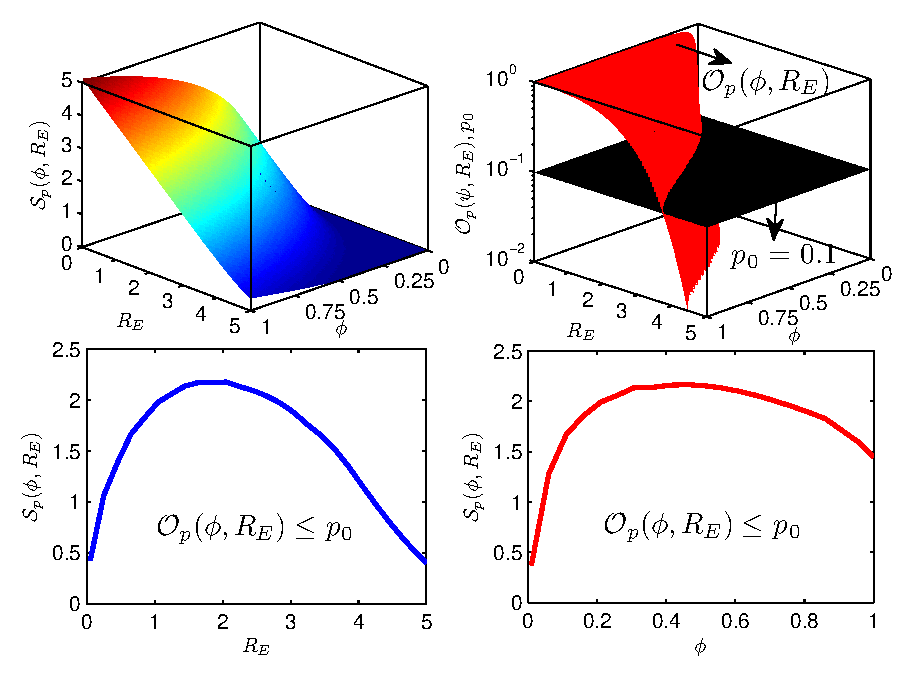
\includegraphics[width=3.5in, height=2.9in]{partial_opt_nogrid.eps}}
    \caption{Average secrecy rate and secrecy outage probability of the partial-adaptive transmission scheme with and without the constraint $P^{so}_p(\phi, R_E) \leq p_0$ for $N = 4$, $M =2$, $\overline{\gamma}_B = 10$dB, $\overline{\gamma}_E = 5$dB, and $p_0 = 0.1$. }\label{fig:opt_partial}
    \end{center}
\end{figure}


For any given $\phi$, both $\mathcal{R}_p (\phi, R_E)$ and $P^{so}_p(\phi, R_E)$ are monotonic decreasing functions of $R_E$, which is confirmed in Fig.~\ref{fig:opt_partial}. As such, for any given $\phi$ the optimal value of $R_E$ is the minimum one that guarantees $P^{so}_p(\phi, R_E) = p_0$. This means that $P^{so}_p(\phi, R_E) = p_0$ is always guaranteed in such optimization, which determines a function between $R_E$ and $\phi$. Then, the two-dimension optimization problem presented in \eqref{opt_partial} can be reduced to a one-dimension optimization problem. We can adopt griding numerical search to solve the optimization problem, in which we first set a value for $\phi$ all over $0< \phi \leq 1$ and then increase $R_E$ until we have $P^{so}_p(\phi, R_E) = p_0$. In Fig.~\ref{fig:opt_partial}, we confirm that $\phi^{\dag}$ and $R_E^{\dag}$ are unique for each pair of $\overline{\gamma}_B$ and $\overline{\gamma}_E$. To facilitate the numerical search, we are more interested in deriving a closed-form expression for $R_E$ in terms of $\phi$ since we know the value range of $\phi$. We would like to highlight that such a closed-form expression can be achieved for the following asymptotic scenarios.

\begin{corollary}
For $M = 1$, as $N \rightarrow \infty$ the optimal $R_E$ for a given $\phi$ is given by
\begin{align}\label{R_E_phi1}
R_E^{\prime} (\phi) = \log_2\left(1-\frac{\phi \overline{\gamma}_E \ln p_0}{(1-\phi)\overline{\gamma}_E + 1}\right).
\end{align}
\end{corollary}
\begin{IEEEproof}
For $M = 1$, as $N \rightarrow \infty$ the CDF of $\gamma_E$ can be approximated as
\begin{align}
F_{\gamma_{E}}\left(\gamma\right) \approx 1 - e^{-\left(\frac{1-\phi}{\phi} + \frac{1}{\phi \overline{\gamma}_E}\right) \gamma}.
\end{align}
Then, by setting $P^{so}_p(\phi, R_E) = p_0$ we achieve the desirable result in \eqref{R_E_phi1}.
\end{IEEEproof}

\begin{corollary}
For $M = 1$, as $\overline{\gamma}_E \rightarrow \infty$ the optimal $R_E$ for a given $\phi$ is given by
\begin{align}
R_E^{\prime} (\phi) = \log_2\left(1+\frac{\phi (N-1) \left(p_0^{{1}/{(1-N)}}-1\right)}{1-\phi}\right).
\end{align}
\end{corollary}





\subsection{Fully-Adaptive Transmission Scheme}

In the fully-adaptive transmission scheme, both $\phi$ and $R_E$ are adaptively chosen for each $\widetilde{\gamma}_B = \overline{\gamma}_B \|\mathbf{f}\|^2$. We also choose $R_B$ as $R_B = C_B$ and thus we have that the instantaneous secrecy rate is a function of $\phi$ and $R_E$, which is given by
\begin{align}\label{Rs_fully}
R_s(\phi, R_E) = [C_B \!-\! R_E]^{+} = \left[\log_2(1+\phi \widetilde{\gamma}_B) \!-\! R_E\right]^{+}.
\end{align}
Alice only transmit signals when $R_s(\phi, R_E) >0$. Thus, the transmission probability of the fully-adaptive transmission scheme is
\begin{align}
P^{tx}_f(\phi, R_E) = \Pr(C_B > R_E) = 1-F_{\gamma_B}\left(2^{R_E}-1\right).
\end{align}
Similar to the partial-adaptive transmission scheme, the secrecy outage probability of the fully-adaptive transmission scheme is
\begin{align}
P^{so}_f(\phi, R_E) = \Pr(C_E > R_E) = 1\!-\!F_{\gamma_E}\left(2^{R_E}\!-\!1\right).
\end{align}

In the fully-adaptive transmission scheme, we intend to maximize the instantaneous secrecy rate $R_s(\phi, R_E)$ for each $\widetilde{\gamma}_B$ subject to a given secrecy outage probability. Then, the optimization problem in the fully-adaptive transmission scheme is given by
\begin{align}\label{opt_fully}
(\phi^{\ddag}, R_E^{\ddag}) \!=\! \argmax_{0< \psi \leq 1, 0< R_E< C_B} R_s (\phi, R_E), ~\text{s.t.}~ \mathcal{O}_f(\phi, R_E) \leq p_0.
\end{align}

\begin{figure}[!t]
    \begin{center}
   {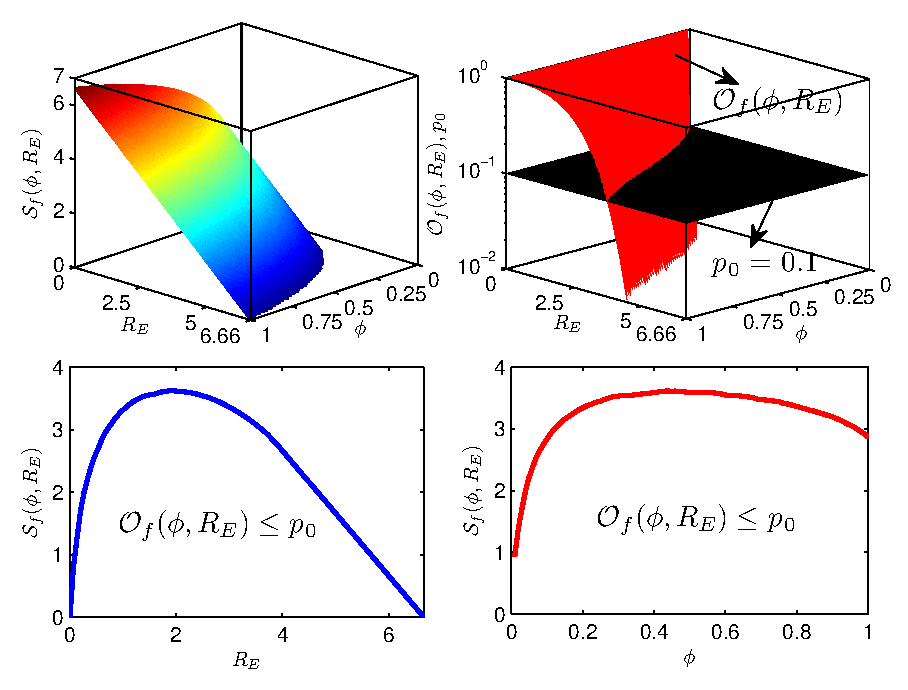
\includegraphics[width=3.5in, height=2.9in]{fully_opt_nogrid.eps}}
    \caption{Average secrecy rate and secrecy outage probability of the fully-adaptive transmission scheme with and without the constraint $P^{so}_f(\phi, R_E) \leq p_0$ for $N = 4$, $M =2$, $\widetilde{\gamma}_B = 20$dB, $\overline{\gamma}_E = 5$dB, and $p_0 = 0.1$. }\label{fig:opt_fully}
    \end{center}
\end{figure}


In Fig.~\ref{fig:opt_fully}, we plot $R_s(\phi, R_E)$ and $P^{so}_f(\phi, R_E)$ with and without the constraint $P^{so}_f(\phi, R_E) \leq p_0$. Again, we confirm that for any given $\phi$ both $R_s$ and $\mathcal{O}_f(\phi, R_E)$ are monotonic decreasing functions of $R_E$. As such, the optimization procedure of the partial-adaptive transmission scheme can be applied to the fully-adaptive transmission scheme and $P^{so}_f(\phi, R_E) = p_0$ is always guaranteed in the optimization presented in \eqref{opt_fully}. Since the optimization is conducted for each $\widetilde{\gamma}_B$, the complexity of the signal processing for the fully-adaptive transmission scheme is much higher than that for the partial-adaptive and on-off transmission schemes. We would like to highlight that $\phi^{\ddag}$ and $R_E^{\ddag}$ can be achieved in closed-from expressions for each $\widetilde{\gamma}_B$ in the following asymptotic scenarios.

\begin{corollary}\label{co02}
For $M = 1$, as $N \rightarrow \infty$ the optimal values of $\phi^{\ast}$ and $R_E^{\ast}$ are given by
\begin{align}
\phi^{\ddag} &= \sqrt{\frac{\ln p_0 \left[(1 + \ln p_0 + \widetilde{\gamma}_B)\overline{\gamma}_E + \widetilde{\gamma}_B\right]}{-\overline{\gamma}_E^2 \widetilde{\gamma}_B (1+\ln p_0)^2(\overline{\gamma}_E + 1)^{-1}}} \!-\! \frac{\overline{\gamma}_E + 1}{\overline{\gamma}_E (1+\ln p_0)},\notag \\
R_E^{\ddag} &= \log_2\left(1-\frac{\phi^{\ddag} \overline{\gamma}_E \ln p_0}{(1-\phi^{\ast})\overline{\gamma}_E + 1}\right).\notag
%R_s^{\ast} & = \log_2 (1+ \phi^{\ast}\widetilde{\gamma}_B) - R_E^{\ast}. \notag
\end{align}
\end{corollary}
\begin{IEEEproof}
Since $P^{so}_f(\phi, R_E) = P^{so}_p(\phi, R_E)$, Corollary~1 is also valid for the fully-adaptive transmission scheme. Substituting \eqref{R_E_phi1} into $R_s(\phi, R_E)$ in \eqref{Rs_fully}, we have
\begin{align}\label{R_s_opt1}
R_s(\phi, R_E^{\dag}(\phi)) \!=\! \log_2 (1 \!+\! \phi \widetilde{\gamma}_B) \!-\! \log_2\left(1\!-\!\frac{\phi \overline{\gamma}_E \ln p_0}{(1\!-\!\phi)\overline{\gamma}_E \!+\! 1}\right).
\end{align}
We first note that we have to guarantee $R_s(\phi, R_E^{\dag}(\phi)) > 0$, which results in
\begin{align}\label{condition}
\widetilde{\gamma}_B > - \frac{\overline{\gamma}_E \ln p_0}{(1-\phi)\overline{\gamma}_E + 1} > - \frac{\overline{\gamma}_E \ln p_0}{\overline{\gamma}_E + 1}.
\end{align}
Following \eqref{R_s_opt1}, we define
\begin{align}\label{g_function}
g(\phi) \triangleq 2^{R_s(\phi, R_E^{\dag}(\phi))} = A \phi + B + \frac{C}{D \phi + E},
\end{align}
where
\begin{align}
A &= \frac{\widetilde{\gamma}_B}{1 + \ln p_0},\notag \\
B &= \frac{\widetilde{\gamma}_B (\overline{\gamma}_E + 1)}{\overline{\gamma}_E (1 + \ln p_0)^2} - \frac{\widetilde{\gamma}_B - \overline{\gamma}_E + \widetilde{\gamma}_B \overline{\gamma}_E}{\overline{\gamma}_E (1 + \ln p_0)}\label{B_definition} \\
C &= (\overline{\gamma}_E + 1)(1-B),\notag \\
D &= -\overline{\gamma}_E (1+\ln p_0),\notag \\
E &= \overline{\gamma}_E + 1.\notag
\end{align}
To maximize $R_s(\phi, R_E^{\dag}(\phi))$ is equivalent to maximize $g(\phi)$. We next prove that $g(\phi)$ is a concave function with respective to $\phi$. Using \eqref{g_function}, we have
\begin{align}
\frac{\partial^2 g(\phi)} {\partial^2 \phi} = \frac{2 D^2 C}{(D \phi + E)^3}.
\end{align}
It is easy to prove that $(D \phi + E)^3 > 0$. Thus, we only have to prove $C < 0$, which means that we have to prove $1-B < 0$ since $C = (\overline{\gamma}_B + 1)(1-B)$ and $\overline{\gamma}_B + 1 >0$. Following \eqref{B_definition}, we have
\begin{align}\label{1_B}
1 - B = \frac{ \overline{\gamma}_E(1+\ln p_0)\ln p_0 + \widetilde{\gamma_B} (1+\overline{\gamma}_E)\ln p_0}{(1+\ln p_0)^2 \overline{\gamma}_E}.
\end{align}
Using \eqref{condition} and noting $p_0<1$, we have
\begin{align}\label{condition1}
\widetilde{\gamma}_B (1+\overline{\gamma}_E) \ln p_0 < - \overline{\gamma}_E (\ln p_0)^2.
\end{align}
Substituting \eqref{condition1} into \eqref{1_B} and noting $p_0<1$, we have
\begin{align}
1-B < \frac{\ln p_0}{(1+\ln p_0)^2} < 0.
\end{align}
As such, we have proved that $g(\phi)$ is a concave function of $\phi$ and we achieve the desirable results presented in Corollary~\ref{co02} by setting $\partial g(\phi)/\partial \phi = 0$.
\end{IEEEproof}

\begin{corollary}
For $M = 1$, as $\overline{\gamma}_E \rightarrow \infty$ the optimal values of $\phi^{\ast}$ and $R_E^{\ast}$ are given by
\begin{align}
\phi^{\ddag} &= \sqrt{\frac{1}{\widetilde{\gamma}_B}\left(\frac{2\widetilde{\gamma}_B }{\alpha - 1} + \frac{\widetilde{\gamma}_B}{(\alpha-1)^2} - 1\right)} - \frac{1}{\alpha - 1},\notag \\
R_E^{\ddag} &= \log_2\left(1-\frac{\phi^{\ddag} \alpha}{(1-\phi^{\ddag})}\right),\notag
\end{align}
where $\alpha$ is given by
\begin{align}
\alpha = (N-1) \left(p_0^{{1}/{(1-N)}}-1\right).
\end{align}
\end{corollary}

We note that the maximum instantaneous secrecy rate $R_s(\phi^{\ddag}, R_E^{\ddag})$ is still a function of $\widetilde{\gamma}_B$. In order to conduct the performance comparison among the three schemes, we have to calculate the average maximum secrecy rate of the fully-adaptive transmission scheme, which is given by
\begin{align}
\mathcal{R}_f^{\ddag} = \int_0^{\infty} R_s(\phi^{\ddag}, R_E^{\ddag}) f_{\widetilde{\gamma}_B}(\widetilde{\gamma}_B) d \widetilde{\gamma}_B,
\end{align}
where $f_{\widetilde{\gamma}_B}(\widetilde{\gamma}_B)$ denotes the pdf of $\widetilde{\gamma}_B$.

\section{Performance Comparison of the Three Different Transmission Schemes}

We present the performance comparison results of the three different transmission schemes in Fig.~\ref{fig:comparison}. We first observe that $\mathcal{R}_p (\phi^{\dag}, R_E^{\dag})$ is much higher than $\mathcal{R}_o (\phi^{\ast}, R_E^{\ast})$, which means that the partial-adaptive transmission scheme dramatically outperforms the on-off transmission scheme. This can be explained by the fact that when the main channel cannot support a fixed secrecy rate $R_s^{\ast}$ under the secrecy constraint in the on-off transmission scheme, a positive secrecy rate $C_B - R_E^{\dag}$ can still be achieved under the secrecy constraint in the partial-adaptive transmission scheme. We would like to highlight that from a wiretap coding perspective point of view the complexity of the partial-adaptive transmission scheme is much lower than that of the on-off transmission scheme. This is due to the fact that both the codeword rate $R_B$ and redundancy rate $R_E$ have to be adjusted for each $\gamma_B$ in the on-off transmission scheme while only the codeword rate $R_B$ varies in the partial-adaptive transmission scheme. In the simulations to obtain Fig.~\ref{fig:comparison}, we confirm that $\mathcal{R}_f^{\ddag}$ is slightly larger than $\mathcal{R}_p (\phi^{\dag}, R_E^{\dag})$, which is not obviously observed in this figure due to the large value range. The minor advantage of the fully-adaptive transmission scheme relative to the partial-adaptive transmission scheme is unexpected (we expect a large advantage since $\phi$ and $R_E$ are adaptively chosen for each instantaneous SNR of the main channel). However, this is reasonable since as per \eqref{condition} we know that a positive secrecy rate is achievable under the secrecy constraint only when $\widetilde{\gamma}_B$ is larger than some specific value, not for every $\widetilde{\gamma}_B$.

\begin{figure}[!t]
    \begin{center}
   {\includegraphics[width=3.5in, height=2.9in]{comparison_nogrid.eps}}
    \caption{Maximum average secrecy rate of the three different transmission schemes for $N = 4$, $M =2$, and $p_0 = 0.1$. }\label{fig:comparison}
    \end{center}
\end{figure}


\begin{thebibliography}{1}

\bibitem{Zhou}
X. Zhou and M. R. McKay,
\newblock ``Secure transmission with artificial noise over fading channels: Achievable rate and optimal power allocation,''
\newblock {\em IEEE Trans. Veh. Technol.}, vol. 59, no. 8, pp. 3831--3842, Oct. 2010.

\bibitem{Gao}
H. Gao, P. J. Smith, and M. V. Clark,
\newblock ``Theoretical reliability of MMSE linear diversity combining in Rayleigh-fading additive interference channels,''
\newblock {\em IEEE Trans. Commun.}, vol. 46, no. 5, pp. 666--672, May 1998.

\end{thebibliography}

\end{document}
